\documentclass{article}
\usepackage{graphicx}
\usepackage{geometry}
\usepackage[MeX]{polski}
\usepackage[polish]{babel}
% Make header with name and date etc.
\usepackage{fancyhdr}
\lhead{Zuzanna Cienka\\nr albumu 148201}
\rhead{\today\\Programowanie obiektowe}
\thispagestyle{fancy}

\usepackage[utf8]{inputenc}
\setlength{\parindent}{0pt} % Don't indent new paragraphs
\setlength{\headheight}{24pt} 

\begin{document}

\begin{center}\vspace{-1cm}
    \textbf{ \huge System rezerwacji biletów lotniczych}\\~\\
    \large Projekt zaliczeniowy C++\\
\end{center}

% \section{Radon Transform of a Gaussian}

% Calculate the Radon transform of $p(\xi, \phi)$ of $f(x,y) = e^{-x^2 - y^2}$. (Hint: there is symmetry you can exploit to simplify this problem).

% \vspace{12pt}
% Program umożliwia użytkownikowi zarezerwowanie biletów lotniczych
Użytkownik ma możliwość wybrać interesujące go połączenie z dwudziestu opcji,
dla dowolnej liczby osób mniejszych od dziesięciu, rezerwując wybrany bilet 
w wersji podstawowej lub biznesowej. Program zawiera trzy klasy: klasę Passenger oraz 
dwie klasy związane z klasami biletów 
lotniczych: klasę Regular oraz klasę Business.


\section*{Klasa Passenger}
Klasa Passenger przechowuje imię, nazwisko, id osoby, miejsce przypisane 
danej osobie oraz cenę biletu dla danej osoby. W klasie Passenger określana 
jest także wielkość zniżki obliczanej na podstawie daty urodzenia danej osoby –
dzieci poniżej 2 lat otrzymują bilet za darmo, a dzieci powyżej 2 lat i poniżej 
18 lat otrzymują zniżkę 40\%.

\section*{Klasy związane z biletami}
Podstawowa wersja biletu – Regular, daje podróżnemu możliwość anulowania lotu 
(kosztującą połowę ceny biletów), zmiany siedzenia podróżnych, przedłużenia 
ważności biletu, dodania dodatkowego bagażu podręcznego oraz zmiany daty odlotu 
(mającą koszt 250 PLN w klasie Regular, i będącą darmową w klasie Business).
Klasy biletów lotniczych 
różnią się tym, że w klasie Regular nie można dodać bagażu innego niż 
podręcznego, a w klasie Business można dodać bagaż zarówno podręczny, 
jak i zwykły. Poza tym w klasie Business jest początkowo możliwe dodanie większej 
ilości bagażu zarówno podręcznego jak i zwykłego. Kolejnymi różnicami w 
obu klasach jest to, że za dodanie większej ilości bagażu w klasie 
Regular trzeba płacić, a w klasie Business – nie. Ponadto, w klasie 
Business, klienci mają możliwość darmowego skorzystania z pobliskiego 
parkingu bez ograniczeń czasowych.

\begin{center}
    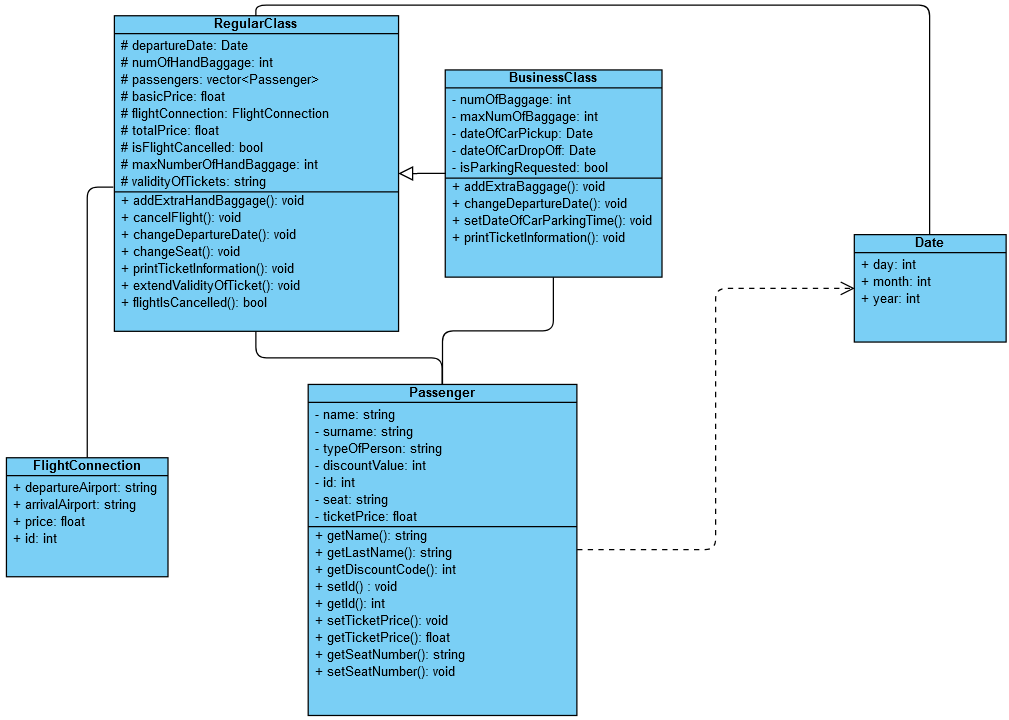
\includegraphics[height=7.1cm]{imgs/1.png}    
\end{center}

\end{document}
